%!TEX root = ../../main.tex

\subsection{What Is A Tensor?} \label{sec:What is A Tensor}
    There is no widely agreed definition of a tensor; different fields define it
    differently. In March 2024, Mathematics Professor Thomas Lam at NYU
    conducted an online informal survey on mathematical conventions
    \cite{Math_Conventions_Survey}. The results of one of its questions can be
    seen on \Cref{fig:What Is A Tensor?}. Though the target audience for
    this survey were mostly mathematicians and mathematics enthusiats, we can
    still observe a lerge variaty in definitions of a tensor. But in the great
    words of my advisor \textit{``84\% of people are wrong''}, and so we reach
    the definition: \textbf{a tensor is a multidimensional array}. 

    \begin{figure}[ht]
        \centering
        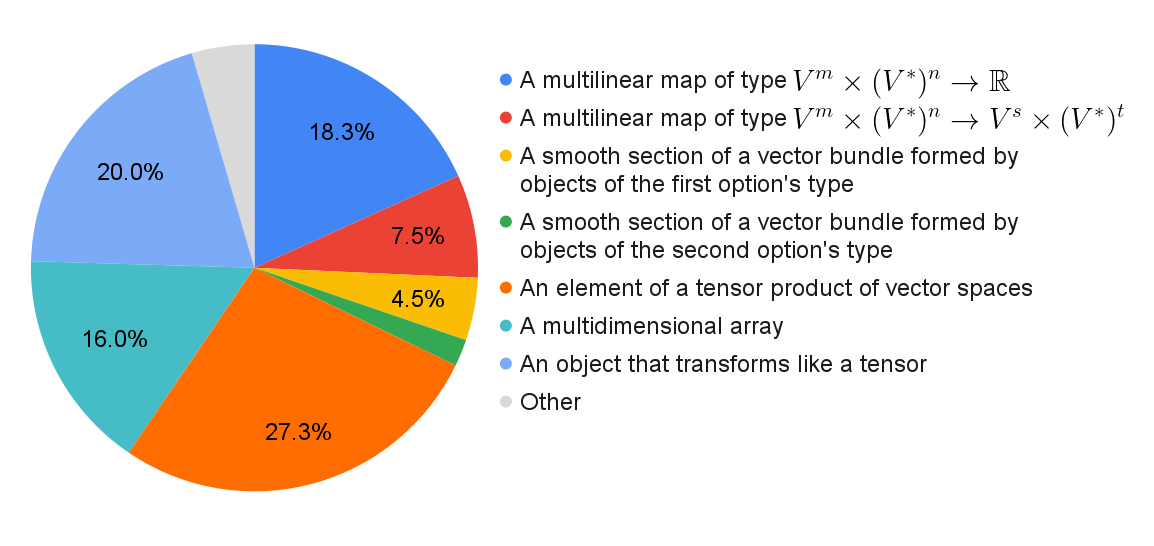
\includegraphics[width=0.8\textwidth, keepaspectratio]{figures/WhatIsATensor.png} % 
        \caption[What Is A Tensor?]{What Is A Tensor?}
        \label{fig:What Is A Tensor?}
    \end{figure}

    In other words, a \textbf{tensor} is a $d$-way array, where $d$ is referred
    to as the order of the tensor. Before we move on any further, a bit of
    notation is required. The set of real values is denoted as $\mathbb{R}$.
    Letters $m, n, p, q, r$ are used to represent sizes (or simply $n_1, \cdots,
    n_d$) and letters $i, j, k, \ell$ are used to represent indices (or simply
    $i_1, \cdots, i_d$). For the sake of simplification, let $[n] \equiv [1,
    \cdots, n]$, and furthermore let $[m] \otimes [n] \equiv \{ (i, j) |
    i\in[m], j\in[n]\}$. Some lower order tensors have other names:


    \begin{itemize}
        \item A \textbf{scalar} is a `zero-dimensional' tensor. This is simply a
        number
        \item A \textbf{vector} is a one-dimensional array of scalars that
        represent a collection of measurements. This can be visualzied on Figure
        \ref{fig:vector}. We represent vectors by lowercase boldface roman
        letters. If $\mathbf{x}$ is a real-valued vector of size $n$, then we
        write that $\mathbf{x} \in \mathbb{R}^n$. Entry $i\in [n]$ of
        $\mathbf{x}$ is denoted as $\mathbf{x}(i)$, or compactly as
        $\mathbf{x}_i$. A vector is a tensor of order 1. Instead of referring to
        them as order 1 tensors, they will simply be referred to as vectors. 
        \item A \textbf{matrix} is a two-dimensional array of numbers, such
        as a collection of vectors This can be vizualized on Figure
        \ref{fig:matrix}. We represent matrices by uppercase boldface roman
        letters. If $\mathbf{X}$ is a real-valued matrix of size $m\times
        n$, then we write $\mathbf{X}\in \mathbb{R}^{m\times n}$. The matrix
        entry $\mathbf{X}(i, j)$ woud represent the $i^\text{th}$ entry of
        vector $j$. More generally, entry $(i, j)\in [m] \otimes [n]$ of
        $\mathbf{X}$ is denoted as $X(i, j)$ or compactly as $\mathbf{x}_{i,
        j}$. A matrix is a tensor of order 2. Instead of referring to
        them as order 2 tensors, they will simply be referred to as matrices.
    \end{itemize}


    \begin{figure}[ht]
        \def\distance{0.2}
        \def\one{0.3}
        \def\n{2}
        \def\m{2.5}
        \def\p{1.5}
        \def\rot{90}

        \centering
        
        % First Subfigure
        \begin{subfigure}[b]{0.26\textwidth}
            \centering
            \begin{tikzpicture}[namenode/.style={scale=1}]

    \coordinate (v) at (0, 0);
    \coordinate (center_v) at ($(\one/2, \n/2)$);

    \coordinate (n_arrow) at ($(v) + (-\distance, \n)$);
    \coordinate (n) at ($(n_arrow) + (-1.25*\distance, -\n/2)$);
    
    \coordinate (one_arrow) at ($(v) + (0, -\distance)$);
    \coordinate (one) at ($(center_v) + (0, -7.5*\distance)$);
    
    \draw[] (v) rectangle (\one, \n);
    \node[namenode] at (center_v) {$\mathbf{x}$};

    \draw[->] (n_arrow) -- (-\distance, 0);
    \node[namenode] at (n) {$n$};
    
    \draw[->] (one_arrow) -- (\one, -\distance);
    \node[namenode] at (one) {$1$};

\end{tikzpicture}x=
            \caption[a Vector]{Vector $\mathbf{x}\in \mathbb{R}^n$ is a 1-way tensor}
            \label{fig:vector}
        \end{subfigure}
        \hfill
        % Second Subfigure
        \begin{subfigure}[b]{0.3\textwidth}
            \centering
            \begin{tikzpicture}[namenode/.style={scale=1}]

    \coordinate (M) at (0, 0);
    \coordinate (center_M) at ($(\m/2, \n/2)$);

    \coordinate (n_arrow) at ($(M) + (-\distance, \n)$);
    \coordinate (n) at ($(n_arrow) + (-1.25*\distance, -\n/2)$);
    
    \coordinate (m_arrow) at ($(M) + (0, -\distance)$);
    \coordinate (m) at ($(center_M) + (0, -7.5*\distance)$);
    
    \draw[] (M) rectangle (\m, \n);
    \node[namenode] at (center_M) {$\mathbf{X}$};

    \draw[->] (n_arrow) -- (-\distance, 0);
    \node[namenode] at (n) {$m$};
    
    \draw[->] (m_arrow) -- (\m, -\distance);
    \node[namenode] at (m) {$n$};

\end{tikzpicture}
            \caption[a Matrix]{Matrix $\mathbf{X} \in \mathbb{R}^{m\times n}$ is a 2-way tensor}
            \label{fig:matrix}
        \end{subfigure}
        \hfill
        % Third Subfigure
        \begin{subfigure}[b]{0.31\textwidth}
            \centering
            \begin{tikzpicture}[namenode/.style={scale=1}]

    \coordinate (M) at (0, 0);
    \coordinate (center_M) at ($(\m/2, \n/2)$);

    \coordinate (n_arrow) at ($(M) + (-\distance, \n)$);
    \coordinate (n) at ($(n_arrow) + (-1.25*\distance, -\n/2)$);
    
    \coordinate (m_arrow) at ($(M) + (0, -\distance)$);
    \coordinate (m) at ($(center_M) + (0, -7.5*\distance)$);
    
    \draw[] (M) rectangle (\m, \n);
    \node[namenode] at (center_M) {$\mathcal{X}$};

    % This scope draws the top face of the cube
    \begin{scope}[shift={(M)}, canvas is zx plane at y=\n,rotate=\rot]
        \draw (0,0) rectangle (\m,\p);
    \end{scope}
    
        % This scope draws the left side of the cube
    \begin{scope}[shift={(M)},canvas is zy plane at x=\m,rotate=90]
        \draw (0,0) rectangle (\n,\p); %
    \end{scope}
    
    \draw[->] (n_arrow) -- (-\distance, 0);
    \node[namenode] at (n) {$m$};
    
    \draw[->] (m_arrow) -- (\m, -\distance);
    \node[namenode] at (m) {$n$};

    \coordinate (p_arrow) at ($(n_arrow) + (\distance, \distance)$);
    \coordinate (p_arrow_end) at ($(p_arrow) + (0.3*\p, 0.3*\p)$);
    \coordinate (p) at (0, 2.5);
    \draw[->] (p_arrow) -- (p_arrow_end);
    \node[namenode] at (p) {$p$};

\end{tikzpicture}
            \caption[a 3D Tensor]{Tensor $\mathcal{X}\in \mathbb{R}^{m\times n \times p}$ is a 3-way tensor}
            \label{fig:tensor3}
        \end{subfigure}

        % Main Figure Caption
        \caption{Tensors of orders one, two, and three}
        \label{fig:Tensors123}
    \end{figure}

    If we have a three-dimensional array of numners, then we have a higher-order
    tensor. Tensors of order 3 or greater are denoted by uppercase mathematical
    caligraphy letters: $\mathcal{X}$. This can be vizualized on Fiugure
    \ref{fig:tensor3}. If $\mathcal{X}$ is a real-valued tensor of size $m\times
    n \times p$, then we write $\mathcal{X}\in \mathbb{R}^{m\times n\times p}$.
    For instance, given a set of $m$ objects, each of which has $n$ features,
    measured under $p$ different scenatios, the tensor entry $\mathcal{X}(i, j,
    k)$ would represent the $j^\text{th}$ feature of object $i$ measured in
    scenario $k$. More generally, entry $(i, j, k) \in [m]\otimes [n]\otimes
    [p]$ of $\mathcal{X}$ is denoted as $X(i, j, k)$ or compactly as
    $x_{i, j, k}$. We refer to each dimension as a \textbf{mode}. Of a
    3-way tensor, we say that mode 1 is of size $m$, mode 2 of size $n$, and
    mode 3 of size $p$. If all modes have the same size, we call this tensor
    \textbf{uniform}.

    As mentioned earlier, any tensor of order greater or equal to three is
    simply referred to as a higher-order tensor. But we begin to run out of
    letters to describe its size and index its modes. This is when we resort
    to subscripts mentioned earlier. \Cref{fig:Tensors45} illustrate
    4-way and 5-way tensors. There, we can visualize the recursive nature of
    tensors. A 4-way tensor is really an array of 3-way tensors, in real
    life that is often used to describe an experiment with three spatial
    dimensions and one time dimension. Similarly, a 5-way tensor is really a
    martrix of 3-way tensors, in real life that is often used to describe an
    experiment with 3 spatial dimensions, one time dimension, and and a
    certain amount of variables being measured is the fifth fimension. To
    remember all of this, Table \ref{tab:tensor_notation}

    % Define a command to draw a single cube
    \newcommand{\drawcube}[1]{
        % These distances can be meddled with to get you what you want
        \def\ix{2} %
        \def\iy{2} %
        \def\iz{1.5} %
        \def\corescale{1}
        \def\rot{90}
        \def\r{0.25} % Thickness of edges
        \def\rx{\ix/\corescale}
        \def\ry{\iy/\corescale}
        \def\rz{\iz/\corescale}

        % Draw the cube
        \begin{tikzpicture}[scale=#1, every node/.style={inner sep=0pt}] % Scale for smaller cubes
            % Define starting point
            \coordinate (TFrontLowerLeft) at (0,0);
            \draw (TFrontLowerLeft) rectangle ++ (\rx,\ry); % Front face

            % Top face
            \begin{scope}[shift={(TFrontLowerLeft)}, canvas is zx plane at y=\ry,rotate=\rot]
            \draw (0,0) rectangle ++ (\rx,\rz);
            \end{scope}

            % Left face
            \begin{scope}[shift={(TFrontLowerLeft)},canvas is zy plane at x=\rx,rotate=\rot]
            \draw (0,0) rectangle ++ (\ry,\rz);
            \end{scope}
        \end{tikzpicture}
    }

    \begin{figure}[ht]
        \centering
        
        % First Subfigure
        \begin{subfigure}[b]{0.49\textwidth}
            \centering
            \[
                \left[
                \begin{array}{c}
                    \drawcube{0.4} \\
                    \vdots \\
                    \drawcube{0.4}
                \end{array}
                \right]
            \]     
            \caption[a 4D Tensor]{A 4D Tensor \newline $\mathcal{X}\in \mathbb{R}^{n_1\times n_2 \times n_3 \times n_4}$}
            \label{fig:tensor4}
        \end{subfigure}
        \hfill
        % Second Subfigure
        \begin{subfigure}[b]{0.49\textwidth}
            \centering
            \[
                \left[
                \begin{array}{ccc}
                    \drawcube{0.4} & \hdots & \drawcube{0.4} \\
                    \vdots & \ddots & \vdots \\
                    \drawcube{0.4} & \hdots & \drawcube{0.4}
                \end{array}
                \right]
            \]
            \caption[a 5D Tensor]{A 5D Tensor \newline $\mathcal{X}\in \mathbb{R}^{n_1\times n_2 \times n_3 \times n_4 \times n_5}$}
            \label{fig:tensor5}
        \end{subfigure}

        % Main Figure Caption
        \caption{Tensors of orders four and five}
        \label{fig:Tensors45}
    \end{figure}

    \begin{table}[ht!]
        \centering
        \renewcommand{\arraystretch}{0.5}
        \begin{tabular}{@{}llcll@{}}
        \toprule
        \textbf{Description} & \textbf{Size} & \textbf{Order} & \textbf{Notation} & \textbf{Entry} \\ 
        \midrule
        Scalar         & $1$                         & $0$ & $x$        & $x$ \\
        Vector         & $n$                         & $1$ & $\mathbf{x}$        & $x(i)$ or $x_i$ \\
        Matrix         & $m \times n$                & $2$ & $\mathbf{X}$        & $X(i,j)$ or $x_{ij}$ \\
        3-way tensor   & $m \times n \times p$       & $3$ & $\mathcal{X}$       & $X(i,j,k)$ or $x_{ijk}$ \\
        4-way tensor   & $n_1 \times n_2 \times n_3 \times n_4$ & $4$ & $\mathcal{X}$ & $X(i_1,i_2,i_3,i_4)$ or $x_{i_1i_2i_3i_4}$ \\
        $d$-way tensor & $n_1 \times n_2 \times \cdots \times n_d$ & $d$ & $\mathcal{X}$ & $X(i_1, i_2, \dots, i_d)$ or $x_{i_1i_2\cdots i_d}$ \\
        \bottomrule
        \end{tabular}
        \caption{Tensor Notation by Order}
        \label{tab:tensor_notation}
    \end{table}

\subsection{Slices and Fibers} \label{sec:Slices and Fibers}
    A slice of a 3-way tensor $\mathcal{X}\in\mathbb{R}^{m\times n\times p}$ is
    a 2-way subtensor (which is a matrix). The $i^\text{th}$ \textbf{horizontal
    slice} is a matrix of size $n \times p$ given by $\mathcal{X}(i, :, :)$. The
    $j^\text{th}$ \textbf{lateral slice} is a matrix of size $m\times n$ given
    by $\mathcal{X}(:, j, :)$. The $k^\text{th}$ \textbf{frontal slice} is a
    matrix of size $m\times n$ given by $\mathcal{X}(:, :, k)$. The three types
    of slices for 3-way tensors are shown in \Cref{fig:slices}

    \begin{figure}[ht]
        \def\distance{0.2}
        \def\m{2.5}
        \def\n{2}
        \def\p{1.5}
        \def\nslices{10}
        \def\rot{90}

        \centering
        
        % First Subfigure
        \begin{subfigure}[b]{0.32\textwidth}
            \centering
            \begin{tikzpicture}[namenode/.style={scale=1}]

    \coordinate (TFrontLowerLeft) at (0, 0);
    
    \draw[] (TFrontLowerLeft) rectangle (\n, \m);

    % This scope draws the top face of the cube
    \begin{scope}[shift={(TFrontLowerLeft)}, canvas is zx plane at y=\m,rotate=\rot]
        \draw (0,0) rectangle (\n,\p);
    \end{scope}
    
    % This scope draws the left side of the cube
    \begin{scope}[shift={(TFrontLowerLeft)},canvas is zy plane at x=\n,rotate=90]
        \draw (0,0) rectangle (\m,\p); %
    \end{scope}

    % Draw slices (horizontal lines) on the front face
    \foreach \i in {1,...,\nslices} {
        \pgfmathsetmacro{\z}{\i*\m/\nslices}
        
        % Draw the lines in front of the cube
        \draw[dashed] (0,\z) -- (\n,\z);

        % Side face (ZY plane) - Shift lines correctly
        \begin{scope}[canvas is zy plane at x=\n]
            \draw[dashed] (0,\z) -- (-\p,\z);
        \end{scope}
    }
    
\end{tikzpicture}
            \caption[Horizontal Slices]{Horizontal Slices $\mathcal{X}(i, :, :)$}
            \label{fig:horizontal_slices}
        \end{subfigure}
        \hfill
        % Second Subfigure
        \begin{subfigure}[b]{0.32\textwidth}
            \centering
            \begin{tikzpicture}[namenode/.style={scale=1}]

    \coordinate (TFrontLowerLeft) at (0, 0);
    
    \draw[] (TFrontLowerLeft) rectangle (\n, \m);

    % This scope draws the top face of the cube
    \begin{scope}[shift={(TFrontLowerLeft)}, canvas is zx plane at y=\m,rotate=\rot]
        \draw (0,0) rectangle (\n,\p);
    \end{scope}
    
    % This scope draws the left side of the cube
    \begin{scope}[shift={(TFrontLowerLeft)},canvas is zy plane at x=\n,rotate=90]
        \draw (0,0) rectangle (\m,\p); %
    \end{scope}

    % Draw slices (horizontal lines) on the front face
    \foreach \i in {1,...,\nslices} {
        \pgfmathsetmacro{\z}{\i*\n/\nslices}
        
        % Draw the lines in front of the cube
        \draw[dashed] (\z,0) -- (\z,\m);

        % Side face (ZY plane) - Shift lines correctly
        \begin{scope}[canvas is zx plane at y=\m]
            \draw[dashed] (0,\z) -- (-\p,\z);
        \end{scope}
    }
    
\end{tikzpicture}
            \caption[Lateral Slices]{Lateral Slices $\mathcal{X}(:, j, :)$}
            \label{fig:lateral_slices}
        \end{subfigure}
        \hfill
        % Third Subfigure
        \begin{subfigure}[b]{0.32\textwidth}
            \def\nslices{6}
            \centering
            \begin{tikzpicture}[namenode/.style={scale=1}]

    \coordinate (TFrontLowerLeft) at (0, 0);
    
    \draw[] (TFrontLowerLeft) rectangle (\n, \m);

    % This scope draws the top face of the cube
    \begin{scope}[shift={(TFrontLowerLeft)}, canvas is zx plane at y=\m,rotate=\rot]
        \draw (0,0) rectangle (\n,\p);
    \end{scope}
    
    % This scope draws the left side of the cube
    \begin{scope}[shift={(TFrontLowerLeft)},canvas is zy plane at x=\n,rotate=90]
        \draw (0,0) rectangle (\m,\p); %
    \end{scope}

    % Draw slices (horizontal lines) on the front face
    \foreach \i in {1,...,\nslices} {
        \pgfmathsetmacro{\z}{\i*\p/\nslices}
        
        % Side face (ZY plane) - Now going TOP to BOTTOM
        \begin{scope}[canvas is zy plane at x=\n]
            \draw[dashed] (-\z,0) -- (-\z,\m);
        \end{scope}

        % Top face (ZX plane) - Now going SIDE to SIDE
        \begin{scope}[canvas is zx plane at y=\m]
            \draw[dashed] (-\z,0) -- (-\z,\n);
        \end{scope}
    }
    
\end{tikzpicture}
            \caption[Frontal Slices]{Frontal Slices $\mathcal{X}(:, :, k)$}
            \label{fig:frontal_slices}
        \end{subfigure}

        % Main Figure Caption
        \caption{Two-way slices of a 3-way tensor}
        \label{fig:slices}
    \end{figure}

    The concept of slices is generalizable for higher-order tensors of order
    greater than or equal to 4, those are called hyperslices. But since that
    goes beyond the scope of this work, it will not be covered here.

    Tensor fibers are the analogs of rows and columns of matrices. The main
    differene between matrx rows and columns and tensor fibers is that tensor
    fibers are always oriented as column vectors when used in calculations. For
    a 3-way tensor, of size $m\times n\times p$, we have the following:

    \begin{itemize}
        \item The \textbf{mode-1 fibers} of length $m$, also known as
        \textbf{column fibers}, range over all indices in the first mode,
        holding the second and third indices fixed. In other words, there are
        $np$ column fibers of the form $\mathbf{x}_{:jk}\in\mathbb{R}^m$. This
        can be vizualized on \Cref{fig:column_fibers}.
        \item The \textbf{mode-2 fibers} of length $m$, also known as
        \textbf{row fibers}, range over all indices in the second mode,
        holding the first and third indices fixed. In other words, there are
        $mp$ row fibers of the form $\mathbf{x}_{i:k}\in\mathbb{R}^n$.This
        can be vizualized on \Cref{fig:row_fibers}.
        \item The \textbf{mode-3 fibers} of length $m$, also known as
        \textbf{tube fibers}, range over all indices in the third mode,
        holding the first and second indices fixed. In other words, there are
        $mn$ tube fibers of the form $\mathbf{x}_{ij:}\in\mathbb{R}^p$. This
        can be vizualized on \Cref{fig:tube_fibers}.
    \end{itemize}

    \begin{figure}[ht]
        \def\m{2.5}
        \def\n{2}
        \def\p{1.5}
        \def\mslices{6}
        \def\nslices{5}
        \def\pslices{4}
        \def\rot{90}

        \centering
        
        % First Subfigure
        \begin{subfigure}[b]{0.32\textwidth}
            \centering
            \begin{tikzpicture}[namenode/.style={scale=1}]

    \coordinate (TFrontLowerLeft) at (0, 0);
    
    \draw[] (TFrontLowerLeft) rectangle (\n, \m);

    % This scope draws the top face of the cube
    \begin{scope}[shift={(TFrontLowerLeft)}, canvas is zx plane at y=\m,rotate=\rot]
        \draw (0,0) rectangle (\n,\p);
    \end{scope}
    
    % This scope draws the left side of the cube
    \begin{scope}[shift={(TFrontLowerLeft)},canvas is zy plane at x=\n,rotate=90]
        \draw (0,0) rectangle (\m,\p); %
    \end{scope}

    % Draw slices (horizontal lines) on the front face
    \foreach \i in {1,...,\nslices} {
        \pgfmathsetmacro{\z}{\i*\n/\nslices}
        
        % Draw the lines in front of the cube
        \draw[ultra thin] (\z,0) -- (\z,\m);

        % Side face (ZY plane) - Shift lines correctly
        \begin{scope}[canvas is zx plane at y=\m]
            \draw[ultra thin] (0,\z) -- (-\p,\z);
        \end{scope}
    }

    % Draw slices (horizontal lines) on the front face
    \foreach \i in {1,...,\pslices} {
        \pgfmathsetmacro{\z}{\i*\p/\pslices}
        
        % Side face (ZY plane) - Now going TOP to BOTTOM
        \begin{scope}[canvas is zy plane at x=\n]
            \draw[ultra thin] (-\z,0) -- (-\z,\m);
        \end{scope}

        % Top face (ZX plane) - Now going SIDE to SIDE
        \begin{scope}[canvas is zx plane at y=\m]
            \draw[ultra thin] (-\z,0) -- (-\z,\n);
        \end{scope}
    }

\end{tikzpicture}
            \caption[Column Fibers]{Column Fibers $\mathbf{x}_{:jk}$}
            \label{fig:column_fibers}
        \end{subfigure}
        \hfill
        % Second Subfigure
        \begin{subfigure}[b]{0.32\textwidth}
            \centering
            \begin{tikzpicture}[namenode/.style={scale=1}]

    \coordinate (TFrontLowerLeft) at (0, 0);
    
    \draw[] (TFrontLowerLeft) rectangle (\n, \m);

    % This scope draws the top face of the cube
    \begin{scope}[shift={(TFrontLowerLeft)}, canvas is zx plane at y=\m,rotate=\rot]
        \draw (0,0) rectangle (\n,\p);
    \end{scope}
    
    % This scope draws the left side of the cube
    \begin{scope}[shift={(TFrontLowerLeft)},canvas is zy plane at x=\n,rotate=90]
        \draw (0,0) rectangle (\m,\p); %
    \end{scope}

    % Draw slices (horizontal lines) on the front face
    \foreach \i in {1,...,\mslices} {
        \pgfmathsetmacro{\z}{\i*\m/\mslices}
        
        % Draw the lines in front of the cube
        \draw[ultra thin] (0,\z) -- (\n,\z);

        % Side face (ZY plane) - Shift lines correctly
        \begin{scope}[canvas is zy plane at x=\n]
            \draw[ultra thin] (0,\z) -- (-\p,\z);
        \end{scope}
    }

    % Draw slices (horizontal lines) on the front face
    \foreach \i in {1,...,\pslices} {
        \pgfmathsetmacro{\z}{\i*\p/\pslices}
        
        % Side face (ZY plane) - Now going TOP to BOTTOM
        \begin{scope}[canvas is zy plane at x=\n]
            \draw[ultra thin] (-\z,0) -- (-\z,\m);
        \end{scope}

        % Top face (ZX plane) - Now going SIDE to SIDE
        \begin{scope}[canvas is zx plane at y=\m]
            \draw[ultra thin] (-\z,0) -- (-\z,\n);
        \end{scope}
    }
    
    
\end{tikzpicture}
            \caption[Row Fibers]{Row Fibers $\mathbf{x}_{i:k}$}
            \label{fig:row_fibers}
        \end{subfigure}
        \hfill
        % Third Subfigure
        \begin{subfigure}[b]{0.32\textwidth}
            \centering
            \begin{tikzpicture}[namenode/.style={scale=1}]

    \coordinate (TFrontLowerLeft) at (0, 0);
    
    \draw[] (TFrontLowerLeft) rectangle (\n, \m);

    % This scope draws the top face of the cube
    \begin{scope}[shift={(TFrontLowerLeft)}, canvas is zx plane at y=\m,rotate=\rot]
        \draw (0,0) rectangle (\n,\p);
    \end{scope}
    
    % This scope draws the left side of the cube
    \begin{scope}[shift={(TFrontLowerLeft)},canvas is zy plane at x=\n,rotate=90]
        \draw (0,0) rectangle (\m,\p); %
    \end{scope}

    % Draw slices (horizontal lines) on the front face
    \foreach \i in {1,...,\mslices} {
        \pgfmathsetmacro{\z}{\i*\m/\mslices}
        
        % Draw the lines in front of the cube
        \draw[ultra thin] (0,\z) -- (\n,\z);

        % Side face (ZY plane) - Shift lines correctly
        \begin{scope}[canvas is zy plane at x=\n]
            \draw[ultra thin] (0,\z) -- (-\p,\z);
        \end{scope}
    }

    % Draw slices (horizontal lines) on the front face
    \foreach \i in {1,...,\nslices} {
        \pgfmathsetmacro{\z}{\i*\n/\nslices}
        
        % Draw the lines in front of the cube
        \draw[ultra thin] (\z,0) -- (\z,\m);

        % Side face (ZY plane) - Shift lines correctly
        \begin{scope}[canvas is zx plane at y=\m]
            \draw[ultra thin] (0,\z) -- (-\p,\z);
        \end{scope}
    }
    
    
\end{tikzpicture}
            \caption[Tube Fibers]{Tube Fibers $\mathbf{x}_{ij:}$}
            \label{fig:tube_fibers}
        \end{subfigure}

        % Main Figure Caption
        \caption{Fibers of a 3-way tensor}
        \label{fig:fibers}
    \end{figure}

\subsection[Tensor Mode-k Unfoldings]{Tensor Mode-$k$ Unfoldings} \label{sec:Tensor Mode k Unfolding}
    The elements of a tensor can be rearranged to form various matrices in a
    procedure referred to as \textbf{unfolding}, also known as
    \textbf{matricization}. A particular unfolding of interest is the mode-$k$
    unfolding which is defined as a matrix whose columns are the mode-$k$ fibers
    of that tensors. The notation for a mode-$k$ unfolding of a tensor
    $\mathcal{X}$ is $\mathbf{X}_{(k)}$. Figure \ref{unfoldings} illustrates the
    mode-$k$ unfoldings of a 3-way tensor.

    \begin{figure}[ht!]
        \def\m{2}
        \def\n{1.5}
        \def\p{1}
        \def\mslices{6}
        \def\nslices{5}
        \def\pslices{4}
        \def\rot{90}

        \centering
        
        % First Subfigure
        \begin{subfigure}[b]{0.24\textwidth}
            \centering
            \begin{tikzpicture}[namenode/.style={scale=1}]

    \coordinate (TFrontLowerLeft) at (0, 0);
    
    \draw[] (TFrontLowerLeft) rectangle (\n, \m);

    \draw[-to, ultra thick] ($(\n/\nslices/2, \m - 0.15)$) -- ($(\n/\nslices/2, 0.15)$);

    % This scope draws the top face of the cube
    \begin{scope}[shift={(TFrontLowerLeft)}, canvas is zx plane at y=\m,rotate=\rot]
        \draw (0,0) rectangle (\n,\p);
    \end{scope}
    
    % This scope draws the left side of the cube
    \begin{scope}[shift={(TFrontLowerLeft)},canvas is zy plane at x=\n,rotate=90]
        \draw (0,0) rectangle (\m,\p); %
    \end{scope}

    % Draw slices (horizontal lines) on the front face
    \foreach \i in {1,...,\nslices} {
        \pgfmathsetmacro{\z}{\i*\n/\nslices}
        
        % Draw the lines in front of the cube
        \draw[ultra thin] (\z,0) -- (\z,\m);

        % Side face (ZY plane) - Shift lines correctly
        \begin{scope}[canvas is zx plane at y=\m]
            \draw[ultra thin] (0,\z) -- (-\p,\z);
        \end{scope}
    }

    % Draw slices (horizontal lines) on the front face
    \foreach \i in {1,...,\pslices} {
        \pgfmathsetmacro{\z}{\i*\p/\pslices}
        
        % Side face (ZY plane) - Now going TOP to BOTTOM
        \begin{scope}[canvas is zy plane at x=\n]
            \draw[ultra thin] (-\z,0) -- (-\z,\m);
        \end{scope}

        % Top face (ZX plane) - Now going SIDE to SIDE
        \begin{scope}[canvas is zx plane at y=\m]
            \draw[ultra thin] (-\z,0) -- (-\z,\n);
        \end{scope}
    }

\end{tikzpicture}
            \caption[Column Fibers]{Mode 1 Fibers}
        \end{subfigure}
        \hfill
        % First Subfigure
        \begin{subfigure}[b]{0.74\textwidth}
            \centering
            \begin{tikzpicture}[namenode/.style={scale=1}]

    \coordinate (TFrontLowerLeft) at (0, 0);
    
    \draw[ultra thick] (TFrontLowerLeft) rectangle (\n*\pslices, \m);

    \draw[-to, ultra thick] ($(\n/\nslices/2, \m - 0.15)$) -- ($(\n/\nslices/2, 0.15)$);

    % Draw slices (horizontal lines) on the front face
    \foreach \i in {1,...,20} {
        \pgfmathsetmacro{\z}{\i*\n/\nslices}
        
        % Draw the lines in front of the cube
        \draw[ultra thin] (\z,0) -- (\z,\m);
        }
        
    \foreach \i in {0,...,4} {
        \pgfmathsetmacro{\z}{\i*\n}
        
        % Draw the lines in front of the cube
        \draw[ultra thick] (\z,0) -- (\z,\m);
    }



\end{tikzpicture}
            \caption[Mode 1 Unfolding]{Mode 1 Unfolding $\mathbf{X}_1$}
        \end{subfigure}

        \vspace{1em}

        % Second Subfigure
        \begin{subfigure}[b]{0.24\textwidth}
            \centering
            \begin{tikzpicture}[namenode/.style={scale=1}]

    \coordinate (TFrontLowerLeft) at (0, 0);
    
    \draw[] (TFrontLowerLeft) rectangle (\n, \m);

    % This scope draws the top face of the cube
    \begin{scope}[shift={(TFrontLowerLeft)}, canvas is zx plane at y=\m,rotate=\rot]
        \draw (0,0) rectangle (\n,\p);
    \end{scope}
    
    % This scope draws the left side of the cube
    \begin{scope}[shift={(TFrontLowerLeft)},canvas is zy plane at x=\n,rotate=90]
        \draw (0,0) rectangle (\m,\p); %
    \end{scope}

    \begin{scope}[shift={(TFrontLowerLeft)}]
        \draw[-to, ultra thick] ($(0.1, \m - \m/\mslices/2)$) -- ($(\n - 0.1, \m - \m/\mslices/2)$);
    \end{scope}

    % Draw slices (horizontal lines) on the front face
    \foreach \i in {1,...,\mslices} {
        \pgfmathsetmacro{\z}{\i*\m/\mslices}
        
        % Draw the lines in front of the cube
        \draw[ultra thin] (0,\z) -- (\n,\z);

        % Side face (ZY plane) - Shift lines correctly
        \begin{scope}[canvas is zy plane at x=\n]
            \draw[ultra thin] (0,\z) -- (-\p,\z);
        \end{scope}
    }

    % Draw slices (horizontal lines) on the front face
    \foreach \i in {1,...,\pslices} {
        \pgfmathsetmacro{\z}{\i*\p/\pslices}
        
        % Side face (ZY plane) - Now going TOP to BOTTOM
        \begin{scope}[canvas is zy plane at x=\n]
            \draw[ultra thin] (-\z,0) -- (-\z,\m);
        \end{scope}

        % Top face (ZX plane) - Now going SIDE to SIDE
        \begin{scope}[canvas is zx plane at y=\m]
            \draw[ultra thin] (-\z,0) -- (-\z,\n);
        \end{scope}
    }
    
    
\end{tikzpicture}
            \caption[Row Fibers]{Mode 1 Fibers}
        \end{subfigure}
        \hfill
        % Second Subfigure
        \begin{subfigure}[b]{0.74\textwidth}
            \centering
            \begin{tikzpicture}[namenode/.style={scale=1}]

    \coordinate (TFrontLowerLeft) at (0, 0);
    
    \draw[ultra thick] (TFrontLowerLeft) rectangle (\m*\pslices, \n);

    % % This scope draws the top face of the cube
    % \begin{scope}[shift={(TFrontLowerLeft)}, canvas is zx plane at y=\m,rotate=\rot]
    %     \draw (0,0) rectangle (\n,\p);
    % \end{scope}
    
    % % This scope draws the left side of the cube
    % \begin{scope}[shift={(TFrontLowerLeft)},canvas is zy plane at x=\n,rotate=90]
    %     \draw (0,0) rectangle (\m,\p); %
    % \end{scope}

    \draw[-to, ultra thick] ($(\m/\mslices/2, \n - 0.15)$) -- ($(\m/\mslices/2, 0.15)$);

    % Draw slices (horizontal lines) on the front face
    \foreach \i in {1,...,24} {
        \pgfmathsetmacro{\z}{\i*\m/\mslices}
        
        % Draw the lines in front of the cube
        \draw[ultra thin] (\z,0) -- (\z,\n);
    }

    \foreach \i in {0,...,4} {
        \pgfmathsetmacro{\z}{\i*\m}
        
        % Draw the lines in front of the cube
        \draw[ultra thick] (\z,0) -- (\z,\n);
    }

    % % Draw slices (horizontal lines) on the front face
    % \foreach \i in {1,...,\pslices} {
    %     \pgfmathsetmacro{\z}{\i*\p/\pslices}
        
    %     % Side face (ZY plane) - Now going TOP to BOTTOM
    %     \begin{scope}[canvas is zy plane at x=\n]
    %         \draw[ultra thin] (-\z,0) -- (-\z,\m);
    %     \end{scope}

    %     % Top face (ZX plane) - Now going SIDE to SIDE
    %     \begin{scope}[canvas is zx plane at y=\m]
    %         \draw[ultra thin] (-\z,0) -- (-\z,\n);
    %     \end{scope}
    % }
    
    
\end{tikzpicture}
            \caption[Row Fibers]{Lateral Slices $\mathbf{X}_2$}
        \end{subfigure}

        \vspace{1em}

        % Third Subfigure
        \begin{subfigure}[b]{0.24\textwidth}
            \centering
            \begin{tikzpicture}[namenode/.style={scale=1}]

    \coordinate (TFrontLowerLeft) at (0, 0);
    
    \draw[] (TFrontLowerLeft) rectangle (\n, \m);

    % This scope draws the top face of the cube
    \begin{scope}[shift={(TFrontLowerLeft)}, canvas is zx plane at y=\m,rotate=\rot]
        \draw (0,0) rectangle (\n,\p);
        \draw[-to, ultra thick] ($(\p/\pslices/2+0.05, 0.1)$) -- ($(\p/\pslices/2+0.05, \p-0.1)$);
    \end{scope}
    
    % This scope draws the left side of the cube
    \begin{scope}[shift={(TFrontLowerLeft)},canvas is zy plane at x=\n,rotate=90]
        \draw (0,0) rectangle (\m,\p); %
    \end{scope}

    % Draw slices (horizontal lines) on the front face
    \foreach \i in {1,...,\mslices} {
        \pgfmathsetmacro{\z}{\i*\m/\mslices}
        
        % Draw the lines in front of the cube
        \draw[ultra thin] (0,\z) -- (\n,\z);

        % Side face (ZY plane) - Shift lines correctly
        \begin{scope}[canvas is zy plane at x=\n]
            \draw[ultra thin] (0,\z) -- (-\p,\z);
        \end{scope}
    }

    % Draw slices (horizontal lines) on the front face
    \foreach \i in {1,...,\nslices} {
        \pgfmathsetmacro{\z}{\i*\n/\nslices}
        
        % Draw the lines in front of the cube
        \draw[ultra thin] (\z,0) -- (\z,\m);

        % Side face (ZY plane) - Shift lines correctly
        \begin{scope}[canvas is zx plane at y=\m]
            \draw[ultra thin] (0,\z) -- (-\p,\z);
        \end{scope}
    }
    
    
\end{tikzpicture}
            \caption[Tube Fibers]{Mode 3 Fibers}
        \end{subfigure}
        \hfill
        % Third Subfigure
        \begin{subfigure}[b]{0.74\textwidth}
            \centering
            \begin{tikzpicture}[namenode/.style={scale=1}]

    \coordinate (TFrontLowerLeft) at (0, 0);
    
    \draw[ultra thick] (TFrontLowerLeft) rectangle (10, \p);

    \draw[-to, ultra thick] ($(\n/\nslices/2, \p - 0.15)$) -- ($(\n/\nslices/2, 0.15)$);

    % Draw slices (horizontal lines) on the front face
    \foreach \i in {1,...,30} {
        \pgfmathsetmacro{\z}{\i*\m/\mslices}
        
        % Draw the lines in front of the cube
        \draw[ultra thin] (\z,0) -- (\z,\p);

        % % Side face (ZY plane) - Shift lines correctly
        % \begin{scope}[canvas is zx plane at y=\m]
        %     \draw[ultra thin] (0,\z) -- (-\p,\z);
        % \end{scope}
    }
    
    \foreach \i in {0,...,5} {
        \pgfmathsetmacro{\z}{\i*\m}
        
        % Draw the lines in front of the cube
        \draw[ultra thick] (\z,0) -- (\z,\p);

        % % Side face (ZY plane) - Shift lines correctly
        % \begin{scope}[canvas is zx plane at y=\m]
        %     \draw[ultra thin] (0,\z) -- (-\p,\z);
        % \end{scope}
    }
    
\end{tikzpicture}
            \caption[Tube Fibers]{Frontal Slices $\mathbf{X}_3$}
        \end{subfigure}

        % Main Figure Caption
        \caption{Unfoldings of a 3-way tensor}
        \label{unfoldings}
    \end{figure}

\subsection{Types of Tensor Multiplication} \label{sec:Types of Tensor Multiplication}
    There are several types of Tensor operations, most of which won't be covered
    here as they go beyond the scope of this work. There are some types of
    products however that are relevant for us. Since multiplication involves two
    objects, the purpose of this subsection is journey through the possible
    types of multiplication increase the number of dimensions of each side of
    the multiplication one at a time. The first few are trivial and can be
    explained briefly. Multiplication of two tensors of order zero is trivial,
    after all you are simply multiplying two scalars. Increasing the dimension
    of one side of the multiplication while fixing the other gets us a
    multiplition of an order zero tensor by an order one tensor (a vector). In
    this product, we are simply \textit{scaling} the entries of the vector by
    the scalar (hence the name). Moving on, we get to products of two tensors of
    order 1, i.e. vector-vector products. There are actually two types of
    products in this scenario the inner product and the outer product which are
    explained below. Though there are also definition for other types of
    products for the scenarios that follow, we will refrain from defining those
    here. As we parse through these types of multiplications, there are two important
    concepts that arise. The \textit{matching} of the dimensions, and the
    \textit{contraction} of these matching dimensions, more on that later.

    \subsubsection{Vector Inner Products} \label{sec:Vector Inner Products}
        Starting small, the inner product of two same-sized vectors $\mathbf{a,
        b} \in \mathbb{R}^n$ produces a scalar, and is denoted as $\langle
        \mathbf{a, b}\rangle = \mathbf{a}^\intercal \mathbf{b}$, and is defined
        as in equation \ref{eq:vec_inner_prod}. A vector norm is defined as the
        inner product of a vector with itself: $\langle \mathbf{a, a} \rangle$.
        The computational complexity of vector inner products is
        $\mathcal{O}(n)$
        \begin{equation} \label{eq:vec_inner_prod}
            \langle \mathbf{a, b} \rangle = \mathbf{a}^\intercal \mathbf{b} = 
            \left[
                \begin{array}{ccc}
                    a_1 & \cdots & a_n
                \end{array} 
            \right]
            \left[
                \begin{array}{c}
                    b_1 \\
                    \vdots \\
                    b_n
                \end{array} 
            \right]
            =
            \sum_{i = 1}^{n} a_ib_i
        \end{equation}
    

    \subsubsection{Vector Outer Products} \label{sec:Vector Outer Products}
        In contrast to vector inner products are a reductive operation which
        generates a scalar, vector outer products are an expansive operation
        which generates a matrix. Vector outer products are defined for multiple
        vectors, which is why we avoid the common notaion of
        $\mathbf{a}^\intercal\mathbf{b}$. So we start by showing the outer
        products of two vectors. Given two vectors $\mathbf{a}\in \mathbb{R}^n$
        and $\mathbf{b}\in \mathbb{R}^m$, their vector outer product is defined
        in equation \ref{eq:vec_outer_prod}. The outer product of two vectors,
        generates a two-dimensional tensor. In general, the outer product of $d$
        vectors, generates a $d$-way tensor, and it is written as $\mathcal{X} =
        \mathbf{x}_1 \circ \cdots \circ \mathbf{x}_d$. The computational
        complexity of the outer product of two vectors of size $m$ and $n$
        respectively is $\mathcal{O}(mn)$. In general, the computational
        complexity of $d$ vectors of respective size of $n_1, \cdots, n_d$ is
        $\mathcal{O}(\prod_{i=1}^{d} n_d)$.

        \begin{align} \label{eq:vec_outer_prod}
            \mathbf{C} & = \mathbf{a} \circ \mathbf{b} \in \mathbb{R}^{m \times n}, \text{ where } c_{ij} = a_i b_j \text{, }\forall(i,j) \in [m] \times [n] \\
            \left[
                \begin{array}{ccc}
                    a_1b_1 & \cdots & a_1b_n \\
                    \vdots & \ddots & \vdots \\
                    a_mb_1 & \cdots & a_mb_n
                \end{array}
            \right]
            & =
            \left[
                \begin{array}{c}
                    a_1 \\
                    \vdots \\
                    a_m
                \end{array}
            \right]
            \left[
                \begin{array}{ccc}
                    b_1 & \cdots & b_n
                \end{array}
            \right] \nonumber
        \end{align}


    \subsubsection{Matrix-Vector Products} \label{sec:Matrix-Vector Products}
        Given a matrix $\mathbf{A}\in \mathbb{R}^{m\times n}$ and vector
        $\mathbf{x}\in \mathbf{R}^n$, the matrix-vector product is defined in
        equation \ref{eq:mat_vec_prod}. The computational complexity of the
        matrix-vector product is $\mathcal{O}(mn)$.

        \begin{align} \label{eq:mat_vec_prod}
            \mathbf{y} & = \mathbf{Ax} \in \mathbb{R}^{m}, \text{ where } y_i = \sum_{j=1}^{n}a_{ij}x_j \text{ for all } i \in [m] \\
            \left[
                \begin{array}{c}
                    a_{11}x_1 + \cdots + a_{1n}x_n \\
                    \vdots \\
                    a_{m1}x_1 + \cdots + a_{mn}x_n
                \end{array}
            \right]
            & =
            \left[
                \begin{array}{ccc}
                    a_{11} & \cdots & a_{1n} \\
                    \vdots & \ddots & \vdots \\
                    a_{m1} & \cdots & a_{mn}
                \end{array}
            \right]
            \left[
                \begin{array}{c}
                    x_1 \\
                    \vdots \\
                    x_n
                \end{array}
            \right] \nonumber
        \end{align}
    

    \subsubsection{Matrix-Matrix Products} \label{sec:Matrix-Matrix Products}
        Given two matrices $\mathbf{A} \in \mathbb{R}^{m\times p}$ and
        $\mathbf{B} \in \mathbb{R}^{p\times n}$, the matrix-matrix product is
        defined in equation \ref{eq:mat_mat_prod}. The computational complexity
        of the matrix-matrix product is $\mathcal{O}(mnp)$. In general, the
        computational complexity of multiplying to same-sized matrices of size
        $n$ by $n$ is $\mathcal{O}(n^3)$. A simple and yet noteworthy example
        can be seen at \ref{eq:two_by_two_mat_mul}, which shows that matrix
        multiplication is performed by inner product of the rows of $\mathbf{A}$
        with the columns of $\mathbf{B}$ for every row of $\mathbf{A}$, for every column of
        $\mathbf{B}$. 

        \begin{equation} \label{eq:mat_mat_prod}
            \mathbf{C = AB}\in \mathbb{R}^{m\times n} \text{, where } c_{ij} = \sum_{k=1}^{p} a_{ik}b_{kj}\text{, } \forall (i, j) \in [m]\otimes [n]
        \end{equation}

        \begin{equation} \label{eq:two_by_two_mat_mul}
            \left[
                \begin{array}{cc}
                    a_{11} & a_{12} \\
                    a_{21} & a_{22}
                \end{array}
            \right]
            \left[
                \begin{array}{cc}
                    b_{11} & b_{12} \\
                    b_{21} & b_{22}
                \end{array}
            \right]
            =
            \left[
                \begin{array}{cc}
                    a_{11}b_{11} + a_{12}b_{21} & a_{11}b_{12} + a_{12}b_{22} \\
                    a_{21}b_{11} + a_{22}b_{21} & a_{21}b_{12} + a_{22}b_{22}
                \end{array}
            \right]
        \end{equation}


    \subsubsection{Tensor-Times-Matrix (TTM) Products} \label{sec:Tensor-Times-Matrix Products}
        The tensor-times-matrix (TTM) product is a mode-wise multiplication
        denoted as $\mathcal{Y} = \mathcal{X}\times_k\mathbf{A}$ where
        $\mathcal{X}$ is a tensor, $k$ is the mode for the TTM, and $\mathbf{A}$
        is a matrix. This product can be transformed into a matrix-matrix
        product using tensor unfoldings, as we can define the product as
        $\mathbf{Y}_{(k)} = \mathbf{AX}_{(k)}$. As the columns of a mode-$k$
        unfolding are the fibers of mode $k$, we can also interpret the TTM
        product in terms of the matrix acting on the fibers. In other words, the
        TTM multiplies each mode-$k$ fibers of $\mathcal{X}$ by $\mathbf{A}$.
        Take a look for example at \Cref{fig:Mode-1_TTM}, in
        \ref{fig:mode1_ttm_matrix_format} we see the notion that a TTM multiply
        each column fiber of $\mathcal{X}$ by the rows of A, and in
        \ref{fig:mode1_ttm_matrix_format} we see the notion that this is
        equivalent to unfolding the input and output tensors and performing a
        regular matrix multiplication.

        \def\m{2.25}
        \def\n{1.25}
        \def\p{1.25}
        \def\q{1}
        \def\r{2.5}
        \def\s{0.75}
        \def\mslices{5}
        \def\nslices{3}
        \def\pslices{4}
        \def\rot{90}
        \def\namedistance{0.3}
        \def\distance{0.2}
        \def\arrowdistancex{0.1}
        \def\arrowdistancey{0.25}
        \begin{figure}[ht]

            \centering
            
            % First Subfigure
            \begin{subfigure}[b]{0.99\textwidth}
                \centering
                \begin{tikzpicture}[namenode/.style={scale=1}]

    \coordinate (YFrontLowerLeft) at (0, 0);
    \coordinate (Ynamenoe) at ($(YFrontLowerLeft) + (\n/2, -\namedistance)$);
    
    \draw (YFrontLowerLeft) rectangle (\n, \q);

    \node[namenode] at (Ynamenoe) {$\mathcal{Y}\in \mathbb{R}^{q\times n \times p}$};

    % This scope draws the top face of the cube
    \begin{scope}[shift={(YFrontLowerLeft)}, canvas is zx plane at y=\q,rotate=\rot]
        \draw (0,0) rectangle (\p,\n);
    \end{scope}
    
    % This scope draws the left side of the cube
    \begin{scope}[shift={(YFrontLowerLeft)},canvas is zy plane at x=\n,rotate=90]
        \draw (0,0) rectangle (\q,\p); %
    \end{scope}

    % Draw slices (horizontal lines) on the front face
    \foreach \i in {1,...,\nslices} {
        \pgfmathsetmacro{\z}{\i*\n/\nslices}
        
        % Draw the lines in front of the cube
        \draw[ultra thin] (\z,0) -- (\z,\q);

        % Side face (ZY plane) - Shift lines correctly
        \begin{scope}[canvas is zx plane at y=\q]
            \draw[ultra thin] (0,\z) -- (-\p,\z);
        \end{scope}
    }

    % Draw slices (horizontal lines) on the front face
    \foreach \i in {1,...,\pslices} {
        \pgfmathsetmacro{\z}{\i*\p/\pslices}
        
        % Side face (ZY plane) - Now going TOP to BOTTOM
        \begin{scope}[canvas is zy plane at x=\n]
            \draw[ultra thin] (-\z,0) -- (-\z,\q);
        \end{scope}

        % Top face (ZX plane) - Now going SIDE to SIDE
        \begin{scope}[canvas is zx plane at y=\q]
            \draw[ultra thin] (-\z,0) -- (-\z,\n);
        \end{scope}
    }

    \coordinate (equal_sign) at ($(YFrontLowerLeft) + (\n + \p/2 + 0.1, \q/2)$);
    \node[namenode] at (equal_sign) {$=$};
    
    \coordinate (ALowerLeft) at ($(YFrontLowerLeft) + (\n + \p/2 + 0.2 + \distance, 0)$);
    \draw (ALowerLeft) rectangle ($(ALowerLeft) + (\m, \q)$);
    \draw[-to, ultra thick] ($(ALowerLeft) + (\arrowdistancex, \q - \arrowdistancey)$) -- ($(ALowerLeft) + (\m - \arrowdistancex, \q - \arrowdistancey)$);

    \coordinate (Anamenode) at ($(ALowerLeft) + (\m/2, -\namedistance)$);
    \node[namenode] at (Anamenode) {$\mathbf{A}\in \mathbb{R}^{q\times m}$};

    
    \coordinate (XFrontLowerLeft) at ($(ALowerLeft) + (\m + \distance, -\m + \q)$);
    \draw (XFrontLowerLeft) rectangle ($(XFrontLowerLeft) + (\n, \m)$);
    
    \coordinate (Xnamenode) at ($(XFrontLowerLeft) + (\n/2, -\namedistance)$);
    \node[namenode] at (Xnamenode) {$\mathcal{X}\in \mathbb{R}^{m\times n\times p}$};

    % This scope draws the top face of the cube
    \begin{scope}[shift={(XFrontLowerLeft)}, canvas is zx plane at y=\m,rotate=\rot]
        \draw (0,0) rectangle (\p,\n);
    \end{scope}
    
    % This scope draws the left side of the cube
    \begin{scope}[shift={(XFrontLowerLeft)},canvas is zy plane at x=\n,rotate=90]
        \draw (0,0) rectangle (\m,\p); %
    \end{scope}

    \begin{scope}[shift={(XFrontLowerLeft)}]
        \draw[-to, ultra thick] ($(\n/\nslices/2, \m - \arrowdistancey)$) -- ($(\n/\nslices/2, \arrowdistancey)$);
    \end{scope}
    
    \begin{scope}[shift={(XFrontLowerLeft)}]
        % Draw slices (horizontal lines) on the front face
        \foreach \i in {1,...,\nslices} {
            \pgfmathsetmacro{\z}{\i*\n/\nslices}
            
            % Draw the lines in front of the cube
            \draw[ultra thin] (\z,0) -- (\z,\m);
    
            % Side face (ZY plane) - Shift lines correctly
            \begin{scope}[canvas is zx plane at y=\m]
                \draw[ultra thin] (0,\z) -- (-\p,\z);
            \end{scope}
        }
    
        % Draw slices (horizontal lines) on the front face
        \foreach \i in {1,...,\pslices} {
            \pgfmathsetmacro{\z}{\i*\p/\pslices}
            
            % Side face (ZY plane) - Now going TOP to BOTTOM
            \begin{scope}[canvas is zy plane at x=\n]
                \draw[ultra thin] (-\z,0) -- (-\z,\m);
            \end{scope}
    
            % Top face (ZX plane) - Now going SIDE to SIDE
            \begin{scope}[canvas is zx plane at y=\m]
                \draw[ultra thin] (-\z,0) -- (-\z,\n);
            \end{scope}
        }
    \end{scope}

\end{tikzpicture}
                \caption[Mode 1 TTM Tensor Format]{Tensor form: the first row of $\mathbf{A}$ and first mode-1 fiber of $\mathcal{X}$ are emphasized with arrows.}
                \label{fig:mode1_ttm_tensor_format}
            \end{subfigure}
            
            \vspace{1em}
            
            % Second Subfigure
            \begin{subfigure}[b]{0.99\textwidth}
                \centering
                \begin{tikzpicture}[namenode/.style={scale=1}]

    \coordinate (YFrontLowerLeft) at (0, 0);
    \coordinate (Ynamenode) at ($(\n*\pslices/2, -\namedistance)$);
    
    \draw (YFrontLowerLeft) rectangle (\n*\pslices, \q);

    % Draw slices (horizontal lines) on the front face
    \foreach \i in {1,...,12} {
        \pgfmathsetmacro{\z}{\i*\n/\nslices}
        
        % Draw the lines in front of the cube
        \draw[ultra thin] (\z,0) -- (\z,\q);
    }

    \node[namenode] at (Ynamenode) {$\mathbf{Y}_{(1)}\in \mathbb{R}^{q\times np}$};

    \coordinate (equal_sign) at ($(YFrontLowerLeft) + (\n*\pslices + \distance + 0.1, \q/2)$);
    \node[namenode] at (equal_sign) {$=$};
    
    \coordinate (ALowerLeft) at ($(YFrontLowerLeft) + (\n*\pslices + 2.15*\distance + 0.2, 0)$);
    \draw (ALowerLeft) rectangle ($(ALowerLeft) + (\m, \q)$);

    \coordinate (Anamenode) at ($(ALowerLeft) + (\m/2, -\namedistance)$);
    \node[namenode] at (Anamenode) {$\mathbf{A}\in \mathbb{R}^{q\times m}$};
    
    \coordinate (XFrontLowerLeft) at ($(ALowerLeft) + (\m + \distance, -\m + \q)$);
    
    \begin{scope}[shift={(XFrontLowerLeft)}]
        \coordinate (Xnamenode) at ($(\n*\pslices/2, -\namedistance)$);
        \node[namenode] at (Xnamenode) {$\mathbf{X}_{(1)} \in \mathbb{R}^{m\times np}$};

        \draw (0,0) rectangle (\n*\pslices, \m);
    
        % Draw slices (horizontal lines) on the front face
        \foreach \i in {1,...,12} {
            \pgfmathsetmacro{\z}{\i*\n/\nslices}
            
            % Draw the lines in front of the cube
            \draw[ultra thin] (\z,0) -- (\z,\m);
        }
    \end{scope}

\end{tikzpicture}
                \caption[Mode 1 TTM Tensor Format]{Matrix form.}
                \label{fig:mode1_ttm_matrix_format}
            \end{subfigure}

            % Main Figure Caption
            \caption[Mode-1 TTM]{Mode-1 TTM (along column fibers)}
            \label{fig:Mode-1_TTM}
        \end{figure}

        Theoretically, this is all that TTM is, but in practice things get more
        difficult. Mode-1 TTMs really are as simple as what the figure conveys,
        but for other modes the way the tensor is stored in memory has a huge
        impact on the way we perform the TTM. The details of how to do so are
        omitted in this work, but if you wish to go understand these finer
        aspects of how TTMs are performed in practice, I recommend you check out
        \cite{Big_Boss}. Because of this omission, \Cref{fig:Mode-2_TTM}
        showcases the theoretical way of performing a TTM on mode 2, which isn't
        how such is performed computationally. Similarly to mode-1 TTM, we can
        either visualize it in its tensor format in
        \ref{fig:mode2_ttm_tensor_format} as applying the matrix $\mathbf{A}$ to
        the row fibers of $\mathcal{X}$. Notice how $A$ is transposed here, this
        is a side effect of TTMs performed in any mode that is not the first and
        the last of its tensor. If we wish to visualize this TTM as matrix
        multiplication, the transpose goes away, and
        \Cref{fig:mode2_ttm_matrix_format} has the same format as
        \Cref{fig:mode1_ttm_matrix_format}.

        \begin{figure}[ht!]
            \centering
            
            % First Subfigure
            \begin{subfigure}[b]{0.99\textwidth}
                \centering
                \begin{tikzpicture}[namenode/.style={scale=1}]

    \coordinate (YFrontLowerLeft) at (0, 0);
    \coordinate (Ynamenoe) at ($(YFrontLowerLeft) + (\r/2, -\namedistance)$);
    
    \draw (YFrontLowerLeft) rectangle (\r, \m);

    \node[namenode] at (Ynamenoe) {$\mathcal{Y}\in \mathbb{R}^{m\times r \times p}$};

    % This scope draws the top face of the cube
    \begin{scope}[shift={(YFrontLowerLeft)}, canvas is zx plane at y=\m,rotate=\rot]
        \draw (0,0) rectangle (\r,\p);
    \end{scope}
    
    % This scope draws the left side of the cube
    \begin{scope}[shift={(YFrontLowerLeft)},canvas is zy plane at x=\r,rotate=90]
        \draw (0,0) rectangle (\m,\p); %
    \end{scope}

    % Draw slices (horizontal lines) on the front face
    \foreach \i in {1,...,\mslices} {
        \pgfmathsetmacro{\z}{\i*\m/\mslices}
        
        % Draw the lines in front of the cube
        \draw[ultra thin] (0,\z) -- (\r,\z);

        % Side face (ZY plane) - Shift lines correctly
        \begin{scope}[canvas is zy plane at x=\r]
            \draw[ultra thin] (0,\z) -- (-\p,\z);
        \end{scope}
    }

    % Draw slices (horizontal lines) on the front face
    \foreach \i in {1,...,\pslices} {
        \pgfmathsetmacro{\z}{\i*\p/\pslices}
        
        % Side face (ZY plane) - Now going TOP to BOTTOM
        \begin{scope}[canvas is zy plane at x=\r]
            \draw[ultra thin] (-\z,0) -- (-\z,\m);
        \end{scope}

        % Top face (ZX plane) - Now going SIDE to SIDE
        \begin{scope}[canvas is zx plane at y=\m]
            \draw[ultra thin] (-\z,0) -- (-\z,\r);
        \end{scope}
    }

    \coordinate (equal_sign) at ($(YFrontLowerLeft) + (\r + \p/2 + 0.1, \m/2)$);
    \node[namenode] at (equal_sign) {$=$};

    
    \coordinate (XFrontLowerLeft) at ($(YFrontLowerLeft) + (\r + \p/2 + \distance + 0.2, -\m + \m)$);
    \draw (XFrontLowerLeft) rectangle ($(XFrontLowerLeft) + (\n, \m)$);
    
    \coordinate (Xnamenode) at ($(XFrontLowerLeft) + (\n/2, -\namedistance)$);
    \node[namenode] at (Xnamenode) {$\mathcal{X}\in \mathbb{R}^{m\times n\times p}$};

    % This scope draws the top face of the cube
    \begin{scope}[shift={(XFrontLowerLeft)}, canvas is zx plane at y=\m,rotate=\rot]
        \draw (0,0) rectangle (\p,\n);
    \end{scope}
    
    % This scope draws the left side of the cube
    \begin{scope}[shift={(XFrontLowerLeft)},canvas is zy plane at x=\n,rotate=90]
        \draw (0,0) rectangle (\m,\p); %
    \end{scope}

    \begin{scope}[shift={(XFrontLowerLeft)}]
        \draw[-to, ultra thick] ($(\arrowdistancex, \m - \m/\mslices/2)$) -- ($(\n - \arrowdistancex, \m - \m/\mslices/2)$);
    \end{scope}
    
    \begin{scope}[shift={(XFrontLowerLeft)}]
        % Draw slices (horizontal lines) on the front face
        \foreach \i in {1,...,\mslices} {
            \pgfmathsetmacro{\z}{\i*\m/\mslices}
            
            % Draw the lines in front of the cube
            \draw[ultra thin] (0,\z) -- (\n,\z);

            % Side face (ZY plane) - Shift lines correctly
            \begin{scope}[canvas is zy plane at x=\n]
                \draw[ultra thin] (0,\z) -- (-\p,\z);
            \end{scope}
        }

        % Draw slices (horizontal lines) on the front face
        \foreach \i in {1,...,\pslices} {
            \pgfmathsetmacro{\z}{\i*\p/\pslices}
            
            % Side face (ZY plane) - Now going TOP to BOTTOM
            \begin{scope}[canvas is zy plane at x=\n]
                \draw[ultra thin] (-\z,0) -- (-\z,\m);
            \end{scope}

            % Top face (ZX plane) - Now going SIDE to SIDE
            \begin{scope}[canvas is zx plane at y=\m]
                \draw[ultra thin] (-\z,0) -- (-\z,\n);
            \end{scope}
        }
    \end{scope}

    \coordinate (ALowerLeft) at ($(XFrontLowerLeft) + (\n + \p/2.5 + \distance, \m - \p/1.65)$);
    \draw (ALowerLeft) rectangle ($(ALowerLeft) + (\r, \n)$);
    \draw[-to, ultra thick] ($(ALowerLeft) + (\arrowdistancex+0.1, \n - \arrowdistancey+0.1)$) -- ($(ALowerLeft) + (\arrowdistancex+0.1, \arrowdistancey-0.1)$);

    \coordinate (Anamenode) at ($(ALowerLeft) + (\r/2, -\namedistance)$);
    \node[namenode] at (Anamenode) {$\mathbf{A}^\intercal\in \mathbb{R}^{n\times r}$};

\end{tikzpicture}
                \caption[Mode 2 TTM Tensor Format]{Tensor form: the first row of $\mathbf{A}$ and first mode-2 fiber of $\mathcal{X}$ are emphasized with arrows.}
                \label{fig:mode2_ttm_tensor_format}
            \end{subfigure}
            
            \vspace{1em}
            
            % Second Subfigure
            \begin{subfigure}[b]{0.99\textwidth}
                \centering
                \begin{tikzpicture}[namenode/.style={scale=1}]

    \coordinate (YFrontLowerLeft) at (0, 0);

    \coordinate (Ynamenode) at ($(\m*\pslices/2, \r + \namedistance)$);
    \node[namenode] at (Ynamenode) {$\mathbf{Y}_{(2)}\in \mathbb{R}^{r\times mp}$};
    
    \draw (YFrontLowerLeft) rectangle (\m*\pslices, \r);

    % Draw slices (horizontal lines) on the front face
    \foreach \i in {1,...,20} {
        \pgfmathsetmacro{\z}{\i*\m/\mslices}
        
        % Draw the lines in front of the cube
        \draw[ultra thin] (\z,0) -- (\z,\r);
    }


    \coordinate (equal_sign) at ($(YFrontLowerLeft) + (\m*\pslices/2, -1.5*\namedistance)$);
    \node[namenode] at (equal_sign) {$=$};
    
    \coordinate (ALowerLeft) at ($(YFrontLowerLeft) + (-\n/2 - \distance/2, -\r -3*\namedistance)$);
    \begin{scope}[shift={(ALowerLeft)}]
        \draw (0, 0) rectangle (\n, \r);
        \coordinate (Anamenode) at ($(\n/2, -\namedistance)$);
        \node[namenode] at (Anamenode) {$\mathbf{A}\in\mathbb{R}^{r\times n}$};

        \coordinate (XLowerLeft) at ($(\n + \distance, \r-\n)$);
        \draw (XLowerLeft) rectangle ($(XLowerLeft) + (\m*\pslices, \n)$);
        \coordinate (Xnamenode) at ($(XLowerLeft) + (\m*\pslices/2, -\namedistance)$);
        \node[namenode] at (Xnamenode) {$\mathbf{X}_{(2)} \in \mathbb{R}^{n \times mp}$};

        \begin{scope}[shift={(XLowerLeft)}]
        % Draw slices (horizontal lines) on the front face
        \foreach \i in {1,...,20} {
            \pgfmathsetmacro{\z}{\i*\m/\mslices}
            
            % Draw the lines in front of the cube
            \draw[ultra thin] (\z,0) -- (\z,\n);
        }
        \end{scope}
    \end{scope}
\end{tikzpicture}
                \caption[Mode 2 TTM Tensor Format]{Matrix Form}
                \label{fig:mode2_ttm_matrix_format}
            \end{subfigure}

            % Main Figure Caption
            \caption[Mode-2 TTM]{Mode-2 TTM (along row fibers)}
            \label{fig:Mode-2_TTM}
        \end{figure}

        It is in the matrix-multiplication format that one can understand best
        the nature of the details of how TTM operations are performed
        computationally. To provide a small glimpse of it we turn our eyes to
        the mode 3 TTM in \Cref{fig:Mode-3_TTM}. Notice that the matrix
        multiplication format of this TTM in \ref{fig:mode3_ttm_matrix_format}
        have been adapted to have the transpose of all elements involved. This
        is to avoid any memory movement which is deemed expensive. Again, more
        details of this can be found on \cite{Big_Boss}

        \begin{figure}
            \centering
            
            % First Subfigure
            \begin{subfigure}[b]{0.99\textwidth}
                \centering
                \begin{tikzpicture}[namenode/.style={scale=1}]

    \coordinate (YFrontLowerLeft) at (0, 0);
    \coordinate (Ynamenoe) at ($(YFrontLowerLeft) + (\n/2, -\namedistance)$);
    
    \draw (YFrontLowerLeft) rectangle (\n, \m);

    \node[namenode] at (Ynamenoe) {$\mathcal{Y}\in \mathbb{R}^{m\times n \times r}$};

    % This scope draws the top face of the cube
    \begin{scope}[shift={(YFrontLowerLeft)}, canvas is zx plane at y=\m,rotate=\rot]
        \draw (0,0) rectangle (\n,\s);
    \end{scope}
    
    % This scope draws the left side of the cube
    \begin{scope}[shift={(YFrontLowerLeft)},canvas is zy plane at x=\n,rotate=90]
        \draw (0,0) rectangle (\m,\s); %
    \end{scope}

    \foreach \i in {1,...,\mslices} {
        \pgfmathsetmacro{\z}{\i*\m/\mslices}
        
        % Draw the lines in front of the cube
        \draw[ultra thin] (0,\z) -- (\n,\z);

        % Side face (ZY plane) - Shift lines correctly
        \begin{scope}[canvas is zy plane at x=\n]
            \draw[ultra thin] (0,\z) -- (-\s,\z);
        \end{scope}
    }

    % Draw slices (horizontal lines) on the front face
    \foreach \i in {1,...,\nslices} {
        \pgfmathsetmacro{\z}{\i*\n/\nslices}
        
        % Draw the lines in front of the cube
        \draw[ultra thin] (\z,0) -- (\z,\m);

        % Side face (ZY plane) - Shift lines correctly
        \begin{scope}[canvas is zx plane at y=\m]
            \draw[ultra thin] (0,\z) -- (-\s,\z);
        \end{scope}
    }

    \coordinate (equal_sign) at ($(YFrontLowerLeft) + (\n + \p/2 + 0.1, \m/2)$);
    \node[namenode] at (equal_sign) {$=$};

    \coordinate (XFrontLowerLeft) at ($(YFrontLowerLeft) + (\n + \p/2 + 0.2 + \distance, 0)$);
    \draw (XFrontLowerLeft) rectangle ($(XFrontLowerLeft) + (\n, \m)$);
    
    \coordinate (Xnamenode) at ($(XFrontLowerLeft) + (\n/2 + \p/2.75, -\namedistance)$);
    \node[namenode] at (Xnamenode) {$\mathcal{X}\in \mathbb{R}^{m\times n\times p}$};

    % This scope draws the top face of the cube
    \begin{scope}[shift={(XFrontLowerLeft)}, canvas is zx plane at y=\m,rotate=\rot]
        \draw (0,0) rectangle (\p,\n);
        \draw[-to, ultra thick] ($(\p/\pslices/2+0.05, \arrowdistancey-0.05)$) -- ($(\p/\pslices/2+0.05, \p-\arrowdistancey+0.05)$);


        \coordinate (ALowerLeft) at ($(0, \p + \distance+0.2)$);
        \draw (ALowerLeft) rectangle ($(ALowerLeft) + (\p, \s)$);
        \draw[-to, ultra thick] ($(ALowerLeft) + (\arrowdistancex+0.025, \arrowdistancex+0.2)$) -- ($(ALowerLeft) + (\p-\arrowdistancex-0.025, \arrowdistancex+0.2)$);
    \end{scope}
    
    \node[namenode] at ($(XFrontLowerLeft) + (1.35*\n, \m+\p)$) {$\mathbf{A}\in\mathbb{R}^{s\times p}$};
    % This scope draws the left side of the cube
    \begin{scope}[shift={(XFrontLowerLeft)},canvas is zy plane at x=\n,rotate=90]
        \draw (0,0) rectangle (\m,\p); %
    \end{scope}
    
    \begin{scope}[shift={(XFrontLowerLeft)}]
        \foreach \i in {1,...,\mslices} {
            \pgfmathsetmacro{\z}{\i*\m/\mslices}
            
            % Draw the lines in front of the cube
            \draw[ultra thin] (0,\z) -- (\n,\z);
    
            % Side face (ZY plane) - Shift lines correctly
            \begin{scope}[canvas is zy plane at x=\n]
                \draw[ultra thin] (0,\z) -- (-\p,\z);
            \end{scope}
        }
    
        \foreach \i in {1,...,\nslices} {
            \pgfmathsetmacro{\z}{\i*\n/\nslices}
            
            % Draw the lines in front of the cube
            \draw[ultra thin] (\z,0) -- (\z,\m);
    
            % Side face (ZY plane) - Shift lines correctly
            \begin{scope}[canvas is zx plane at y=\m]
                \draw[ultra thin] (0,\z) -- (-\p,\z);
            \end{scope}
        }
    
    \end{scope}

\end{tikzpicture}
                \caption[Mode 2 TTM Tensor Format]{Tensor form: the first row of $\mathbf{A}$ and first mode-3 fiber of $\mathcal{X}$ are emphasized with arrows.}
                \label{fig:mode3_ttm_tensor_format}
            \end{subfigure}
            
            \vspace{1em}
            
            % Second Subfigure
            \begin{subfigure}[b]{0.99\textwidth}
                \centering
                \begin{tikzpicture}[namenode/.style={scale=1}]

    \coordinate (YFrontLowerLeft) at (0, 0);
    \coordinate (Ynamenode) at ($(\s/2, \m*\nslices+\namedistance)$);
    
    \draw (YFrontLowerLeft) rectangle (\s, \m*\nslices);
    \node[namenode] at (Ynamenode) {$\mathbf{Y}^\intercal_{(3)} \in\mathbb{R}^{mn\times s}$};

    % Draw slices (horizontal lines) on the front face
    \foreach \i in {1,...,15} {
        \pgfmathsetmacro{\z}{\i*\m/\mslices}
        
        % Draw the lines in front of the cube
        \draw[ultra thin] (0,\z) -- (\s,\z);
    }

    \coordinate (equal_sign) at ($(YFrontLowerLeft) + (\s + 6*\distance + 0.1, \m*\nslices/2)$);
    \node[namenode] at (equal_sign) {$=$};
    
    % \coordinate (ALowerLeft) at ($(YFrontLowerLeft) + (\n*\pslices + 2.15*\distance + 0.2, 0)$);
    % \draw (ALowerLeft) rectangle ($(ALowerLeft) + (\m, \q)$);

    % \coordinate (Anamenode) at ($(ALowerLeft) + (\m/2, -\namedistance)$);
    % \node[namenode] at (Anamenode) {$\mathbf{A}\in \mathbb{R}^{q\times m}$};
    
    \coordinate (XFrontLowerLeft) at ($(YFrontLowerLeft) + (\s + 12*\distance + 0.2, 0)$);
    
    \begin{scope}[shift={(XFrontLowerLeft)}]
        \coordinate (Xnamenode) at ($(\p/2, \m*\nslices+\namedistance)$);
        \node[namenode] at (Xnamenode) {$\mathbf{X}_{(3)}^\intercal \in \mathbb{R}^{mn\times p}$};

        \draw (0,0) rectangle (\p, \m*\nslices);
    
        % Draw slices (horizontal lines) on the front face
        \foreach \i in {1,...,15} {
            \pgfmathsetmacro{\z}{\i*\m/\mslices}
            
            % Draw the lines in front of the cube
            \draw[ultra thin] (0,\z) -- (\p,\z);
        }

        \coordinate (ALowerLeft) at ($(XFrontLowerLeft) + (\p + \distance, \m*\nslices - \p)$);
        \draw (ALowerLeft) rectangle++ (\s, \p);
        \coordinate (Anamenode) at ($(ALowerLeft) + (\s + 3.5*\namedistance, \p/2)$);
        \node[namenode] at (Anamenode) {$\mathbf{A}^\intercal \in \mathbb{R}^{p\times s}$};
    \end{scope}

\end{tikzpicture}
                \caption[Mode 3 TTM Tensor Format]{Matrix Form}
                \label{fig:mode3_ttm_matrix_format}
            \end{subfigure}

            % Main Figure Caption
            \caption[Mode-3 TTM]{Mode-3 TTM (along tube fibers)}
            \label{fig:Mode-3_TTM}
        \end{figure}

    
    \subsubsection{Tensor-Times-Tensor (TTT) products} \label{sec:Tensor-Times-Tensor Products}
        The last type of Tensor multiplication required for this work is the
        Tensor-Times-Tensor (TTT) multiplication, which is also known as Tensor
        Contraction. Before diving in to this one which is fairly difficult to
        visualize by the means of drawing as we have been seeing so far, it is
        worth taking a step back to reflect on the types of multiplication
        already covered.

        Notice how from the very first type of multiplication, we needed the
        \textit{inner dimensions to match}. For 1D tensors, arrays, There were
        two types of multiplication as there are two ways we can match the
        dimensions. An array $\mathbf{a} \in \mathbb{R}^{n}$ can be multiplied
        by an array $\mathbf{b}$ of the same length either through $a^\intercal
        b$ (inner product) or $ab^\intercal$ (outer product). In other words, we
        could either perform a $1 \times n$ by $n\times 1$ inner product or an
        $n\times 1$ by $1\times n$ outer product. The former \textit{contracts}
        the $n$ vs $n$ dimensions to produce a $1$ by $1$ scalar, and the latter
        \textit{contracts} the $1$ vs $1$ dimensions to produce an $n$ by $n$
        matrix. The same idea of contracting the matching inner dimensions can
        be seen in matrix-vector products where we match the second dimension of
        matrix $\mathbf{A}\in \mathbb{R}^{m\times n}$ to the first dimension of
        vector $\mathbf{x}\in \mathbb{R}^n$, where they are then contracted to
        produce a vector of size $m$. In matrix-multiplication we match the
        inner dimenions of two matrices, contract those two matching dimensions,
        and the size of the output matrix is the outer dimensions of the two
        matrices. In a mode-$k$ TTM we match the columns of matrix to the
        mode-$k$ fibers of a tensor $\mathcal{X}$, then the $k^\text{th}$ mode
        is contracted. The idea of the generalized tensor contraction is the
        same, contract the matching modes of two tensors. 

        Consider two tensors, $\mathcal{X}\in\mathbb{R}^{m\times n\times p}$ and
        $\mathcal{X}\in\mathbb{R}^{p\times q\times r}$. The last mode of
        $\mathcal{X}$ matches the size of the first mode of $\mathcal{Y}$, so we
        can contract along those modes. The result is a tensor
        $\mathcal{Z}\in\mathbb{R}^{m\times n\times q\times r}$ defined by 

        \begin{equation*}
            \mathcal{Z}(i_1, i_2, j_1, j_2) = \sum_{k=1}^{p} \mathcal{X}(i_1, i_2, k)\cdot \mathcal{Y}(k, j_1, j_2)\text{, }\forall (i_1, i_2, j_1, j_2) \in [m]\otimes[n]\otimes[q]\otimes[p]
        \end{equation*}

        As mentioned earlier, the nature of the drawings presented so far are
        not useful for visualizing this form of multiplication, this is where we
        turn to tensor diagrams. Tensor contractions can get complicated not
        only because of this change in visualization, but also in the notation
        for $d$-way tensor contractions. Since the details go beyond the scope
        of this work, they will be omitted. For this work, it suffices to know
        that as long as one or more modes of two tensors match, a contraction is
        possible along those modes. 